\documentclass{report}

\usepackage[utf8]{inputenc}
\usepackage[0T1]{inputenc}
\usepackage{fancyhdr}
\usepackage[french]{babel}
\usepackage{graphicx}
\graphicspath{ { /home/david/outils-libres/ } } 
\pagestyle{fancy}
\fancyhead[L]{David de Deus}
\fancyhead[C]{Compte rendu TP outils libres côtés client}
\fancyhead[R]{\today}

\begin{document}
\chapter{Efficacité}
\section{TP 1}
 
\subsection{raccourci clavier}
\begin{tabular}{|c|c|c|}
	\hline
	\textbf{Numéros} &  \textbf{Problème} & \textbf{Correctif} \\ 
	\hline
	1 & Logout & \textsc{ctrl + alt + del} \\
	\hline
	2 & Verrouiler la session & \textsc{win + l} \\
	\hline  
	3 & Fermer un onglet & \textsc{ctrl-w} \\
	\hline
	4 & Changer d'onglet & \textsc{ctrl + tab}  \\
	\hline
	5 & Suivant ou précédent & \textsc{alt + < ou alt + >} \\
	\hline 
	6 & Ouvrir un nouvel onglet & \textsc{ctrl + t} \\
	\hline
	7 & Ouvrir une nouvelle instance & \textsc{ctrl + n} \\
	\hline 
	8 & Changer de console & \textsc{ctrl + alt + n°console} \\
	\hline 
	9 & Debut de ligne & \textsc{ctrl + a} \\
	\hline 
	10 & Fin de ligne & \textsc{ctrl + e} \\
	\hline 
	11 & Clear le terminal & \textsc{ctrl + l} \\
	\hline 
\end{tabular}

\section{TP 2}
J'ai utilisé le site arckade.fr car il est assez intuitif, on peut aussi
chercher à s'amélioré grâce aux statistique qui sont plutôt bien détaillé.
\\
\\
\newpage
L'interface du site :
\\
\\  
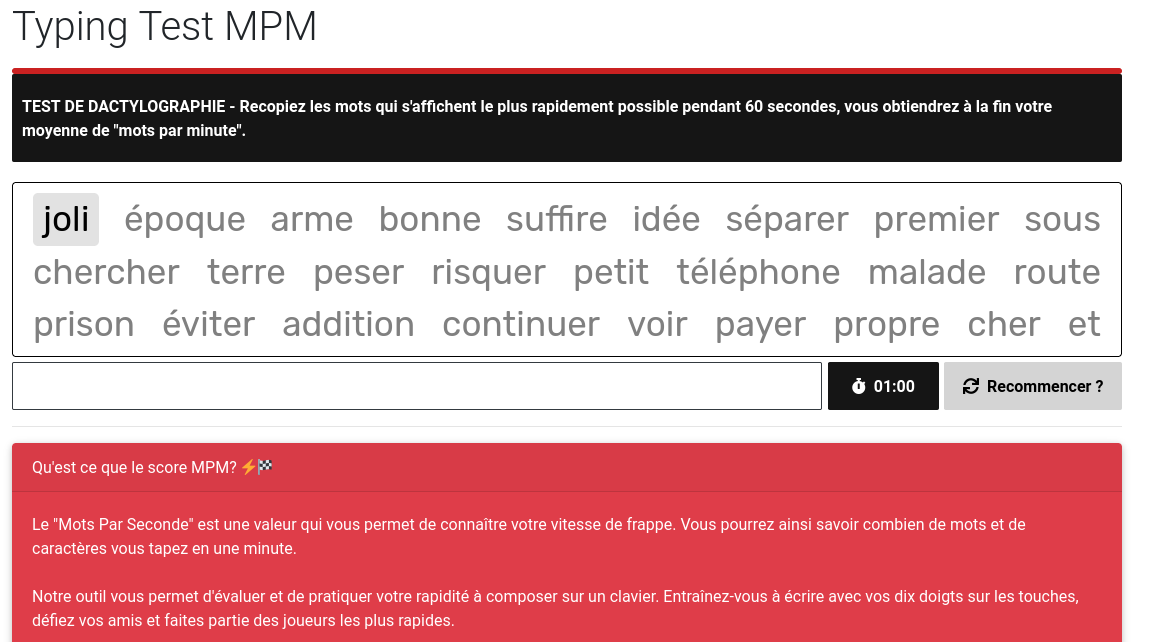
\includegraphics{arckade}
\\
\\
Les statistiques à la fin de chaque test :
\\
\\ 
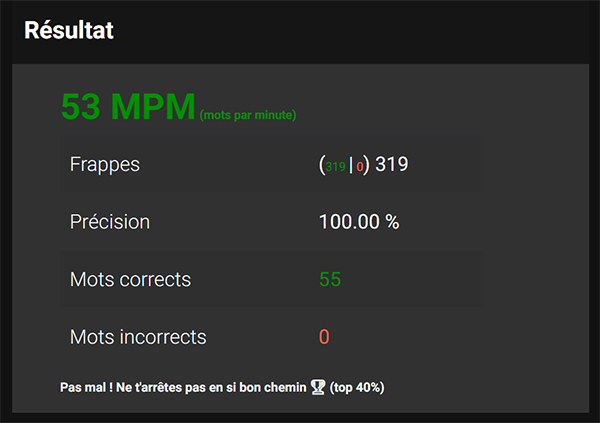
\includegraphics{stats} 
\\
\newpage
\section{TP 4}
On peut voir quelques informations sensibles et on pourrais y rémédier en 
masquant ceci dans l'\textbf{history}.
\\
Ses anciens \textbf{history} peuvent être autre part ou l'employé à 
changé de shell. 
\\
On peut masquer les diffèrentes commandes.
\\
\section{TP 5}
\\
\begin{tabular}{|c|c|}
\hline
\textbf{script mkcd} & \textbf{script gitemergency}\\
\hline
\textit{function mkcd() mkdir -p "\$1" \&\& cd "\$1";} & 
\textit{function gitemergency () git add "\$1" \&\&}\\
\textit{alias mkcd="mkcd"} & \textit{git commit "\$1" \&\&} \\
& \textit{git push "\$1" "\$2"}\\
\hline
\end{tabular}
\\ 
\\
\section{TP 6}
\begin{tabular}{|c|}
\hline
\textit{complete -W "now, tonight, tomorrow" backup.sh}\\
\textit{complete -A directory backup.sh}\\
\textit{complete -A HOME.directory backup.sh}\\
\hline
\end{tabular}
\section{TP 9}
\\
J'ai testé les terminaux Terminator, Sakura et Kitty. 
\\
Ensuite, j'ai choisi Terminator pour sa fonction de redimensionnement qui
est plutôt bien intuitive, sa rapidité est correcte et quand on a plusieurs 
onglets actifs, c'est ergonomique.   
\\
\chapter{SSH}

\section{TP 1}
\\
Pour se connecter sans utiliser \textbf{vagrant ssh}, les commandes à utilisés sont : \\
\\
\begin{tabular}{|c|}
\hline
\textit{ssh alice@10.0.0.3} \\
\textit{ssh bob@10.0.0.3} \\
\textit{ssh carol@10.0.0.3} \\
\hline
\end{tabular}
\\
\\
On est pas en local, car ce n'est pas l'addresse IP du poste local.

\section{TP 2}
\subsection{génération des clés ssh}
\\
\begin{tabular}{|c|}
\hline
\textit{debiandav@david \% ssh-keygen} \\
\hline
\end{tabular}
\\
\subsection{copie des clés ssh}
\\
\begin{tabular}{|c|}
\hline 
\textit{debiandav@david \% sudo ssh-copy ~/.ssh/id\_rsa.pub} \\
\textit{debiandav@david \% sudo ~/.ssh/id\_rsa bob@10.0.0.3:\./cle.txt} \\ 
\textit{debiandav@david \% ssh bob@10.0.0.3} \\
\hline
\textit{bob@srv:~\$ mkdir .ssh} \\
\textit{bob@srv:~\$ cat cle.txt \> ~/.ssh/authorized\_keys} \\
\hline
\end{tabular}
\\

\subsection{définition d'une passphrase}
C'est une phrase pour s'authentifié lors d'une connexion en ssh, 
elle permet ainsi de protéger la clé publique.

\section{TP 3}
\\
\begin{tabular}{|c|}
\hline
\textit{ssh-keyscan -H 10.0.0.3 \> /home/david/.ssh/known\_hosts} \\
\hline
\end{tabular}
\\
\subsection{fichier config}
\\
\begin{tabular}{|c|}
\hline
\textit{touch .ssh/config} \\ 
\textit{sudo chmod 600 .ssh/config} \\
\textit{nano .ssh/config} \\
\hline
\textit{Host bs} \\
\textit{Hostname 10.0.0.3} \\
\textit{Port 22} \\
\textit{User bob} \\
\hline
\end{tabular}
\\
\\
La commande \textbf{ssh bc} fonctionne bien.

\subsection{SFTP}
\\
\begin{tabular}{|c|}
\hline
\textit{debiandav@david ~ \% sftp alice@10.0.0.3} \\
\textit{sftp\> put /home/david/outils\_libres/vagrant/README.md} \\
\textit{sftp\> get /home/bob/cle.pub} \\
\textit{sftp\> exit} \\
\hline
\end{tabular}
\\
\subsection{SSHFS}
\\
\begin{tabular}{|c|}
\hline
\textit{mkdir /tmp/alice\_srv} \\
\hline
\end{tabular}
\\
\\
J'ai mit le fichier à modifier dans ce dossier. \\
\\
\begin{tabular}{|c|}
\hline
\textit{debiandav@david ~ \% sshfs alice@10.0.0.3:/home/alice /tmp/alice\_srv} \\
\textit{debiandav@david ~ \% subl /tmp/alice\_srv/README.md} \\
\hline
\end{tabular}
\\
\\
Avec sublimetext , j'ai effacé tout le contenue en mettant "john". \\
Ensuite on vérifie en se connectant avec alice. \\
\\
\begin{tabular}{|c|}
\hline
\textit{alice@srv:\~\$ cat README.md} \\
\textit{john} \\
\hline
\end{tabular}
\\
\section{TP 4}
\\
\begin{tabular}{|c|}
\hline
\textit{carol@cli:~\$ ssh -L 8000:srv.local:80 carol@cli.local}\\
\hline
\end{tabular}
\\
\section{TP 5}
\\
\begin{tabular}{|c|}
\hline
\textit{ssh -D 9000 carol@cli.local}\\
\textit{tsocks -on}\\
\textit{tsocks firefox}\\
\hline
\end{tabular}
\\
\\
\section{TP 6}
\\
\begin{tabular}{|c|}
\hline
\textit{carol@cli:~\$ apt install x11-app}\\
\textit{carol@cli:~\$ apt install xauth}\\
\textit{debiandav@david ~ \% ssh -X carol@10.0.0.2}\\
\textit{carol@cli:~\$ xeyes}\\
\hline
\end{tabular}
\\
\\
Le xeyes s'affiche bien. 
\\
\\
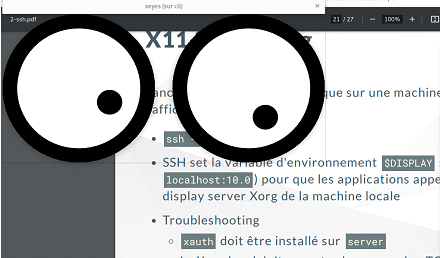
\includegraphics{xeyes}
\\
\\
\section{TP 7}
\begin{tabular}{|c|c|}
\hline
\textbf{ProxyJump} & \textbf{ProxyCommand} \\
\hline 
\textit{Host bastion} & \texit{Host bastion}\\
\textit{Hostname 10.0.0.3} & \textit{Hostname 10.0.0.2}\\
\textit{User bob} & \textit{User bob}\\
\hline
\textit{Host srv} & \textit{Host srvcmd}\\
\textit{Hostname 10.0.0.3} & \textit{Hostname 10.0.0.3}\\
\textit{User bob} & \textit{User bob}\\
\textit{ProxyJump bastion} & \texit{ProxyCommand ssh bastion -W \%h:\%p}\\
\hline
\end{tabular}
\\
   
\chapter{GIT}

\section{TP 1}
on remarque que les fichiers ne sont pas ajoutés au repository donc pour régler le problème 
on commit les modifications apportés.

\subsection{ajout des vagrant files}
\\
\begin{tabular}{|c|}
\hline
\textit{git commit -m "ajout des vagrantfiles"}\\
\textit{[master (commit racine) 0b7a33a] ajout des vagrantfiles} \\
\textit{ 3 files changed, 70 insertions(+)} \\
\textit{ create mode 100644 vagrant/Vagrantfile}\\
\textit{ create mode 100755 vagrant/srv/test1.cgi}\\
\textit{ create mode 100755 vagrant/srv/test2.cgi}\\
\hline
\end{tabular}
\\
\subsection{log commit}
\\
\begin{tabular}{|c|}
\hline
\textit{git log commit 0b7a33a2e6f7c228dceb08d0eb079476ee5a6f26 (HEAD -> master)}\\
\textit{Author: Skoneek3r <david.dedeus@free.fr>}\\
\textit{Date:   Fri Feb 4 15:46:07 2022 +0100 ajout des vagrantfiles}\\
\hline
\end{tabular}
\\
\section{TP 2}
le \textbf{working directory} fonctionne bien mais il n'a pas changé.

la branche crée existe toujours mais on peut la supprimer à l'aide de la commande 
\textbf{git branch -d nom-de-la-branche}

\section{TP 3}
il y a un conflit entre les branches.
\subsection{log final}
\\
\begin{tabular}{|c|}
\hline
\textit{commit d4c33bd6503f98ec1ba2a28adad6428b2ecd660b (HEAD -> forward-new-port)}\\
\textit{Author: Skoneek3r <david.dedeus@free.fr>}\\
\textit{Date:   Fri Feb 4 16:39:56 2022 +0100}\\
\textit{modifié: outils\_libres\_david\_dedeus.tex}\\
\textit{modifié: vagrant/Vagrantfile}\\
\textit{commit 39b9d8d20057f05c82f4fe274321c3c8d3c1ccd3}\\
\textit{Author: Skoneek3r <david.dedeus@free.fr>}\\
\textit{Date:   Fri Feb 4 16:34:45 2022 +0100}\\
\textit{ 8081 pour srv}\\
\textit{commit 0b7a33a2e6f7c228dceb08d0eb079476ee5a6f26 (vagrant, master)}\\
\textit{Author: Skoneek3r <david.dedeus@free.fr>}\\
\textit{Date:   Fri Feb 4 15:46:07 2022 +0100}\\
\textit{    ajout des vagrantfiles}\\
\hline
\end{tabular}
\\

\end{document}
